\chapter{Previous Work}

\section{Specialization Project}
\label{sec:specialization}

A specialization Project was done prior to this thesis called "Designing a RISC-V Reference Model for Open Source Processor Cores" \cite{torjenygaardeikenesDesigningRISCVReference2023}. The report explored different design choices for a cycle-accurate reference model. This section will summarize the relevant findings from the report.




\subsection{Reference Model Architecture}
\label{sec:pw_architecture}

The report proposed a reference model architecture based on the two-layered modeling technique proposed by \textcite{chiangEfficientTwolayeredCycleaccurate2009} and \textcite{leeFaCSimFastCycleAccurate2008} which both use a core-independent untimed functional kernel and a core-dependent timing shell that we will call \gls{ps}.

This architecture comprising of a custom \gls{ps} customized to the specific core, built on top of an existing \acrshort{iss} was chosen instead of building the entire reference model from scratch or modifying an existing microarchitectural simulator. 

This two-layered partitioning allows the \acrshort{iss} to be a functional kernel that is core-independent and is responsible for correct instruction-level functionality described in the \acrshort{isa} specification. 

The \gls{ps} built on top, should only be responsible for the correct timing of the core-specific timing of the user-visible values and side effects generated from the \acrshort{iss}. 

This partitioning enhances the modularity of the system, since only the \gls{ps} needs to be modified for a new core, and the \acrshort{iss} can be easily replaced and updated, without modifying the \gls{ps}. 


\subsection{Pipeline Shell Design}
\label{sec:pw_pipelineShellDesign}

The report proposed two different \gls{ps} designs: a \Gls{stagebased} and a \Gls{timewheel}. 

In the stage-based design, the pipeline is modeled like the actual pipeline, where each stage can hold one instruction and is moved through the pipeline.

The \Gls{timewheel} proposed in \cite{chiangEfficientTwolayeredCycleaccurate2009}, has a \textit{time wheel} with slots for each cycle instead of slots for each pipeline stage and is shown in \cref{fig:time wheel block}. This requires a \textit{commander} that decides when ISS should step through a new instruction, depending on the inputs and time wheel. The results from the \acrshort{iss} is passed into the \textit{scheduler}, that uses the core specific timing details to populate the cycle slots in the \textit{time wheel} with the state changes generated in the ISS. The time wheel advances every cycle, and outputs the last correct cycle to the outputs.

\begin{figure}[htb]
    \centering
    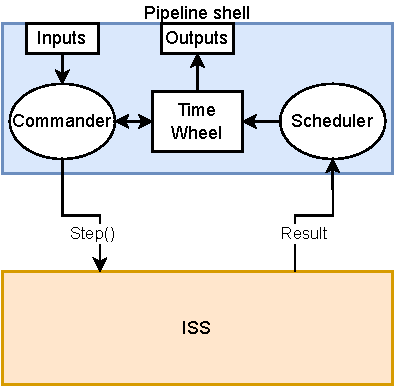
\includegraphics[width=0.5\linewidth]{prosjektoppgave/time-wheel.pdf}
    \caption{Block diagram of the pipeline shell with a cycle-based time wheel approach.}
    \label{fig:time wheel block}
\end{figure}

The report compared the two and some important points will be listed below.

The different slots of the \textit{time wheel} can contain effects from multiple instructions, and a single instructions can have side effects that are spread out over multiple cycle slots. This makes it complicated to manage flushing of some pipeline stages, as situations can arise where only parts of a time wheel slot must be flushed. Using a stage-based approach, flushing and stalling stages are easier since each stage only contains effects from a single instruction.

Another problem is multicycle instructions. Since the time wheel has one slot for each cycle, the scheduler needs to know the number of cycles an instruction will take before inserting it into the wheel. Additionally, the time wheel must be able to hold the worst-case scenario for the number of cycles and instructions in the pipeline, or have a dynamic size. The stage-based approach on the other hand, has a fixed number of slots, equal to the amount of pipeline stages. 

One disadvantage of the stage-based design is that it closely relates to how the core actually works. If both the reference model and the core are modeled the same way, the same bug could be implemented in both and not be detected.


\subsubsection{Abstraction level}

Work was also done to determine the appropriate abstraction level necessary to properly time interrupts. By analyzing the \acrshort{rtl} code of the \gls{cv32x} core, the dependency tree in \cref{fig:dependency-tree-cv32x}. This gives a visual understanding of all the components that affect the timing of an interrupt and can be used when building the reference model.

\begin{figure}[htb]
    \centering
    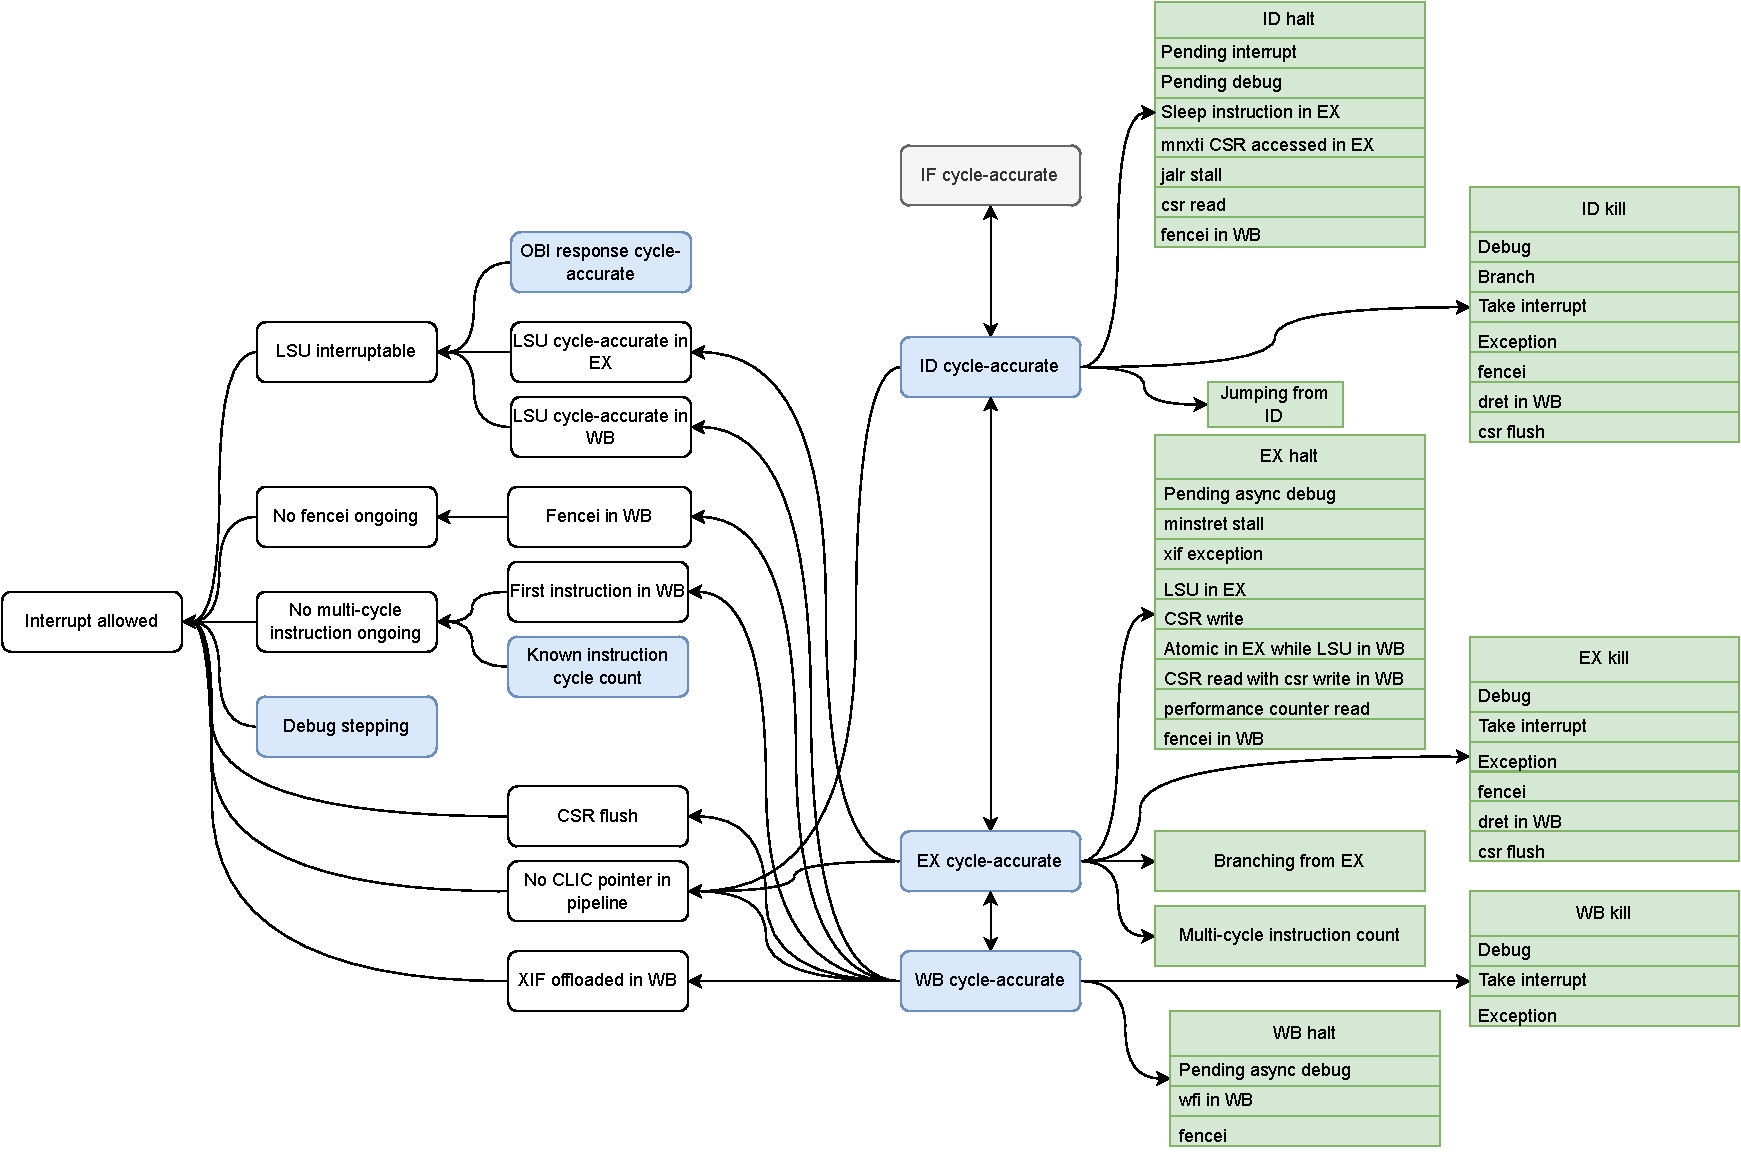
\includegraphics[width=1.0\linewidth]{figures/Dependencies.pdf}
    \caption{Simulation dependency tree for interrupt timing in the \gls{cv32x} core.}
    \label{fig:dependency-tree-cv32x}
\end{figure}

\subsubsection{Pipeline shell and ISS partitioning and interaction}
\label{sec:pw_partition}

The specialization project also evaluated different partitions between the \gls{ps} and \acrshort{iss}. Tree approaches were compared with varying amounts of necessary modifications to the \acrshort{iss}. For side effects to be properly timed, two approaches were discussed that split up the \acrshort{iss} into different stages that are triggered at different points in the pipeline shell. These modifications to the ISS would be invasive, hard to implement, and hard to maintain, so a third approach was proposed that would keep the ISS as intact as possible. In this approach, the ISS would step through a whole instruction and return the state changes to the \acrshort{if} stage in the pipeline shell. Keeping the ISS intact has multiple advantages. Since it executes a full instruction at a time, we do not need to simulate forwarding to keep the data used in instructions correct, but the pipeline shell should instead simulate halts and hazards. Keeping the ISS intact also makes it easier to replace in the future and keep updated. With this approach, all side effects and registers are essentially updated in the \acrshort{if} stage, so the pipeline shell is responsible for timing these changes externally. Additionally, the state of the ISS might have to be reverted to a previous state to handle pipeline flushes caused by interrupts or debug requests. One proposed solution to this is to keep a copy of the register file and \acrshort{csr}s that is written to by the pipeline shell at the correct cycles. During a pipeline flush, the internal register files of the ISS can be reverted to the state of the external register files.


\begin{figure}[htb]
    \centering
    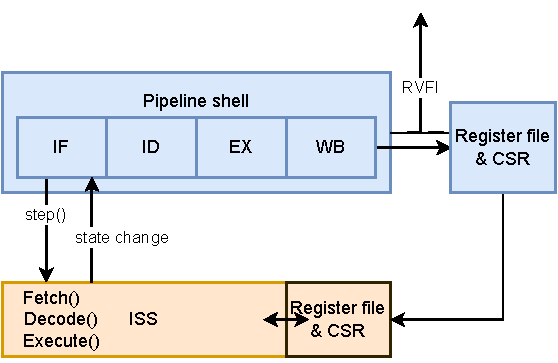
\includegraphics[width=0.5\linewidth]{figures/pipeline-iss-3.pdf}
    \caption{Pipeline and ISS interaction.}
    \label{fig:pipeline-iss-3}
\end{figure}

\subsection{ISS}
\label{sec:pw_iss}

The report compared many different \acrshort{iss}s considering a set of requirements necessary to be used in the reference model, where Spike \cite{SpikeRISCVISA2023} and sail-riscv \cite{RISCVSailModel2023} passed all requirements. They were further compared against each other and found that both are viable options, but Spike is likely easier to get started with and modify, while sail-riscv can be more future-proof as the sail model has been adopted as the golden formal model for \acrshort{riscv}. These will be compared further in this thesis, also considering formal verification.




